\section{Apresentar possíveis parceiros}

\par Esta funcionalidade apresenta ao usuário possíveis parceiros que poderão compor a sua rede de relacionamentos. Para realizar esta busca, também foi preciso escrever uma consulta que levasse em conta dois níveis de análise, sendo elas, a busca pelo possível parceiro dentro da empresa onde o usuário trabalha, levando em conta a quantidade de parceiros em comum entre ambos (usuário autenticado e o possível parceiro) e a busca por parceiros dentro da mesma cidade, também seguindo este mesmo critério. O Código~\ref{list:consulta_possiveis_parceiros} apresenta a \textit{query} utilizada para realizar esta busca.

\par A Figura~\ref{fig:busca_possiveis_parceiros} apresenta o resultado da busca por possíveis parceiros, contendo uma lista com as pessoas que atendam os requisitos pré estabelecidos na consulta.

\begin{figure}[h!]
	\centerline{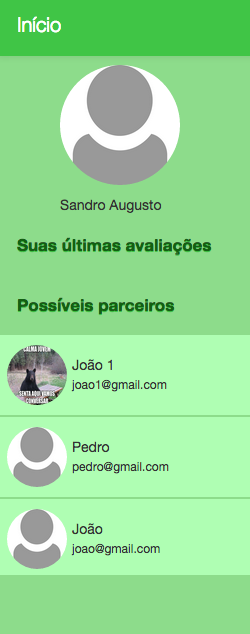
\includegraphics[scale=0.4]{./imagens/busca-possiveis-parceiros.png}}
	\caption[Funcionalidade que apresenta a lista com possíveis parceiros.]
	{Funcionalidade que apresenta a lista com possíveis parceiros. \textbf{Fonte:} Elaborado pelos autores.}
	\label{fig:busca_possiveis_parceiros}
\end{figure}

\par A ideia desta funcionalidade foi apresentar um possível parceiro que provavelmente já tenha algum vínculo com o usuário ou que possua afinidade com alguém da sua rede de parceria.